%!TEX root = Main.tex
\documentclass[Main]{subfiles}

\begin{document}

\section*{Exercise 5}

\paragraph{1. Write out $J(x)$} 
The Jacobian matrix is given by 


$J(x) = \begin{bmatrix}
\dfrac{\partial r_1}{\partial x_1} (x) & \ldots & \dfrac{\partial r_1}{\partial x_n} (x) \\
\vdots & & \vdots \\
\dfrac{\partial r_m}{\partial x_1} (x) & \ldots & \dfrac{\partial r_m}{\partial x_n} (x)
\end{bmatrix}$

This means we can take the derivative regarding the $m$ and $n$-column:

\begin{lstlisting}[caption=J(x), style=Code-Matlab, label=lst:CH5-1]
syms yi A ti s;
r = yi - A*exp(-(ti^2/s^2));
J1 = diff(r, A)
J2 = diff(r, s)
\end{lstlisting}

\begin{align*}
J1 &= -e^{-\dfrac{t_i^2}{s^2}} \\
J2 &= - \dfrac{2 \cdot A \cdot t_i^2 \cdot e^{-\dfrac{ti^2}{s^2}}}{s^3}
\end{align*}



\paragraph{2. Fill in the missing code:}

\begin{lstlisting}[caption=MatLab code, style=Code-Matlab, label=lst:CH5-2]
%Newton Gauss data fitting
%HKa sep. 2013
clear close all  clc;
%simulate dataset
t=(-2:.01:2);
x_gold=[1;.1];
y=x_gold(1)*exp(-(t).^2/x_gold(2)^2);
y=y+.03*randn(size(y));
figure(1)
plot(y,'.b'); 
hold on;
%pause
xx = [];
x = x_gold+[.9;.9];
for k = 1:75
    %Jacobian
    J = [ 
        -exp(-t.^2/x(2)^2) ; 
        -(2*x(1)*t.^2.*exp(-t.^2/x(2)^2))/x(2)^3 ].';
    
    % The function
    f = x(1)*exp(-(t).^2/x(2)^2);
    
    % r
    r = y - f;
    x = x - (J.'*J)^(-1) * (J.' * r.');
    xx = [xx,x];
    plot(f)  
end
figure(2)
plot(xx(1,:),'.r');hold on;
plot(xx(2,:),'.g');
xlabel('Iterations')
\end{lstlisting}


\begin{figure}[hbtp]
\centering
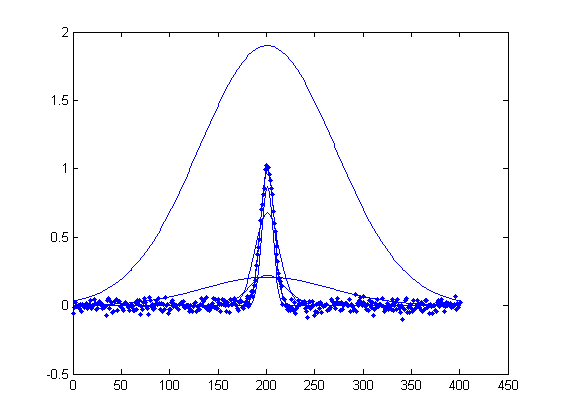
\includegraphics[width = 0.6 \textwidth]{CH5-1}
\vspace{-15pt}
\caption{Data}
\label{fig:CH5-1}
\end{figure}

\begin{figure}[hbtp]
\centering
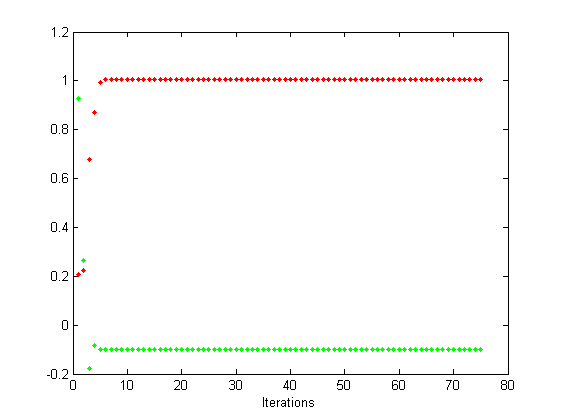
\includegraphics[width = 0.6 \textwidth]{CH5-2}
\vspace{-15pt}
\caption{Iterations}
\label{fig:CH5-2}
\end{figure}









\end{document}